\documentclass[10pt,twocolumn]{article}

% ============================================================================
% PACKAGES
% ============================================================================
\usepackage[utf8]{inputenc}
\usepackage[T1]{fontenc}
\usepackage{times}
\usepackage{graphicx}
\usepackage{amsmath}
\usepackage{amssymb}
\usepackage{booktabs}
\usepackage{multirow}
\usepackage{array}
\usepackage{xcolor}
\usepackage{hyperref}
\usepackage[margin=1in]{geometry}
\usepackage{caption}
\usepackage{subcaption}
\usepackage{float}
\usepackage{enumitem}
\usepackage{url}

% Figures: run plotting cells in notebooks/mrnet_training.ipynb (SAVE_REPORT_FIGURES=True),
% then compile this file from the reports/ directory: pdflatex mrnet_transfer_learning_report.tex
\graphicspath{{figures/}}

% ============================================================================
% DOCUMENT SETTINGS
% ============================================================================
\setlength{\parindent}{1em}
\setlength{\parskip}{0pt}
\linespread{1.1}

\hypersetup{
    colorlinks=true,
    linkcolor=blue,
    citecolor=blue,
    urlcolor=blue
}

% ============================================================================
% TITLE
% ============================================================================
\title{\Large Transfer Learning vs.\ Fine-Tuning on MRNet: \\
Multi-Task Knee MRI Classification with ResNet-18}

\author{
Nicholas Hefner \\
\textit{Department of Computer Engineering and Computer Science} \\
\textit{California State University, Long Beach} \\
\texttt{nicholas.hefner@student.csulb.edu}
}

\date{}

% ============================================================================
% DOCUMENT BEGIN
% ============================================================================
\begin{document}

\maketitle

% ============================================================================
% ABSTRACT
% ============================================================================
\begin{abstract}
Knee MRI diagnosis is constrained by cost, throughput, and inter-reader variability, while demand for knee imaging remains high. This report studies whether transfer learning and fine-tuning can support consistent, automated screening-style classification when labeled clinical volumes are limited. I use the Stanford MRNet dataset~\cite{bien2018plos,bien2020deep,stanford_mrnet} with three binary tasks (abnormality, ACL tear, meniscal tear), a three-branch ResNet-18 architecture with ImageNet-pretrained weights, and multi-plane (axial, coronal, sagittal) fusion. I compare fine-tuning (backbone frozen for one warmup epoch, then unfrozen) against transfer-only training (backbone frozen for all epochs; task heads only). On the official validation split, fine-tuning achieves substantially higher validation AUC on every task; the mean validation AUC across tasks is approximately 0.861 versus 0.628 for transfer-only, a gap of about 0.23. I summarize modeling challenges (domain gap, class imbalance, variable volume size) and limitations: a single configuration, validation-only evaluation, and results tied to one training environment.
\end{abstract}

% ============================================================================
% SECTION 1: INTRODUCTION
% ============================================================================
\section{Introduction}
\label{sec:introduction}

\subsection{Problem and motivation}

Knee injuries are among the most common indications for MRI; accurate interpretation nevertheless depends on subspecialized radiologists, and imaging volume can outpace available expertise. Knee MRI diagnosis is therefore bottlenecked by cost, turnaround time, and human inconsistency. Decision-support models trained on public benchmarks cannot replace clinicians, but can still improve triage consistency and highlight subtle findings if they are validated carefully.

\subsection{Proposed solution and goals}

This project applies transfer learning and multi-task, multi-plane fusion to automate binary classification for three knee conditions on MRNet: abnormality, ACL tear, and meniscal tear. The high-level goals align with a screening-assist setting: reduce excessive reliance on scarce specialists for first-pass scoring, improve consistency across cases, and surface pathology that is easy to miss under time pressure---while acknowledging that deployment would require regulatory and clinical workflows outside this course scope.

\subsection{Research question}

Public benchmarks such as MRNet~\cite{bien2020deep} enable reproducible comparison of modeling choices. A practical design question is how aggressively to adapt an ImageNet-pretrained backbone: training only lightweight heads (transfer-only / linear probing) is fast and stabilizes optimization, whereas fine-tuning updates backbone weights to better match MRI appearance at the cost of fitting more parameters on limited data.

In this coursework experiment, I ask:
\begin{itemize}[noitemsep,topsep=0pt]
    \item How much validation AUC improves when ResNet-18 backbones are fine-tuned vs.\ kept frozen for all epochs?
    \item Whether gains are uniform across MRNet tasks (abnormal, ACL, meniscus).
\end{itemize}

\subsection{Contributions}

\begin{enumerate}[noitemsep,topsep=0pt]
    \item Problem framing and design rationale: clinical motivation, dataset imbalance, and engineering challenges (domain gap, variable-length volumes, multi-plane fusion).
    \item A controlled protocol: identical splits, preprocessing, architecture, epochs, optimizer, and batch size---only backbone training policy differs after initialization.
    \item Quantitative comparison on MRNet validation AUC per task plus mean AUC across tasks, with ROC and learning curves.
    \item A reproducible PyTorch notebook pipeline (\texttt{notebooks/mrnet\_training.ipynb}).
\end{enumerate}

Paper organization.
Section~\ref{sec:background} reviews MRNet, knee MRI volume structure, class imbalance, and transfer learning.
Section~\ref{sec:methodology} describes preprocessing, the fusion architecture, training strategies, and metrics.
Section~\ref{sec:results} reports validation AUCs, figures, and discussion.
Section~\ref{sec:related} highlights related literature.
Section~\ref{sec:conclusion} concludes.

% ============================================================================
% SECTION 2: BACKGROUND
% ============================================================================
\section{Background}
\label{sec:background}

\subsection{MRNet Dataset}

Stanford MRNet provides $1{,}370$ knee MRI exams with binary labels for three clinical conditions~\cite{bien2018plos,bien2020deep, stanford_mrnet}. Standard splits assign roughly $1{,}130$ training, $120$ validation, and $120$ hidden test cases. Each exam includes three orthogonal planes stored as numeric arrays (see below).

Class imbalance is severe and task-dependent. Table~\ref{tab:mrnet_skew} summarizes positive/negative counts on the train and validation splits (from the CSVs used in the notebook pipeline). Abnormality is predominantly positive in training, while ACL tear is rare ($\approx 18\%$ positives in train), which inflates variance for naive accuracy and motivates AUC-based evaluation.

\begin{table}[H]
\centering
\caption{MRNet label skew by task (train / valid splits, counts of positive and negative cases).}
\label{tab:mrnet_skew}
\scriptsize
\setlength{\tabcolsep}{3pt}
\resizebox{\columnwidth}{!}{%
\begin{tabular}{lcccc}
\toprule
Task & Tr.\ pos. & Tr.\ neg. & \% pos. & Val.\,+\,/\,$-$ \\
\midrule
Abnormal  & 913 & 217 & 80.8\% & 95\,/\,25 \\
ACL       & 208 & 922 & 18.4\% & 54\,/\,66 \\
Meniscus  & 397 & 733 & 35.1\% & 52\,/\,68 \\
\bottomrule
\end{tabular}%
}
\end{table}

\subsection{Knee MRI volumes and imaging planes}

Each exam is acquired as three separate stacks of two-dimensional slices: axial (horizontal cross-sections), coronal (front--back), and sagittal (side view). In MRNet, each plane is commonly represented as a stack on the order of $25$--$40$ grayscale slices at $256\times 256$ resolution per slice. Interpreters integrate evidence across planes; the learning system mirrors that requirement through multi-plane fusion rather than a single 2D slice classifier~\cite{bien2020deep}.

\subsection{Transfer Learning and Fine-Tuning}

Transfer learning initializes a network with weights trained on another domain (here, ImageNet) and adjusts parameters on medical data~\cite{deng2009imagenet, he2016deep}.

Transfer-only training freezes early feature extractors and trains only the task-specific head(s), limiting capacity to adapt low-level patterns.

Fine-tuning allows gradient updates to propagate into the backbone, often improving performance when the target domain differs from pretraining, at the cost of more parameters to fit and higher overfitting risk on small datasets.

\subsection{Metrics}

For each binary task, I report validation AUC (area under the ROC curve) using scikit-learn, consistent with ranking-based evaluation on imbalanced medical labels. The competition-style summary uses the mean of the three task AUCs~\cite{bien2020deep}.

% ============================================================================
% SECTION 3: METHODOLOGY
% ============================================================================
\section{Methodology}
\label{sec:methodology}

\subsection{Challenges and design responses}

Building a knee MRI classifier on MRNet introduces challenges highlighted in the project development process; Table~\ref{tab:challenges} maps each issue to the design choice used in the notebook.

\begin{table}[H]
\centering
\caption{Challenges and mitigations in this implementation.}
\label{tab:challenges}
\small
\begin{tabular}{p{0.38\linewidth}p{0.54\linewidth}}
\toprule
Challenge & Mitigation \\
\midrule
Limited supervised data ($\approx$1.1k training exams) &
ImageNet pretraining + careful validation monitoring; transfer-only baseline \\
\midrule
Domain gap (natural images vs.\ MRI) &
Fine-tuning Phase~2; optional longer freezes in future work \\
\midrule
Multi-view reasoning &
Three-branch encoder + fusion before the task logit \\
\midrule
Variable number of slices per exam/plane &
Batch size 1, per-volume aggregation (global max pool across slices) \\
\midrule
Class imbalance (Table~\ref{tab:mrnet_skew}) &
AUC/ROC as primary metrics \\
\midrule
Grayscale MRI vs.\ 3-channel ResNet inputs &
Per-slice replication to three channels before the ImageNet stem \\
\bottomrule
\end{tabular}
\end{table}

\subsection{Data preprocessing}

Unless otherwise noted, the training pipeline follows these steps for each plane's volume:
\begin{itemize}[noitemsep,topsep=0pt]
    \item Load \texttt{.npy} tensors shaped $(S, 256, 256)$ for $S$ slices (slice count varies by patient and plane).
    \item Per-volume min--max normalization to $[0, 1]$.
    \item Resize $256\times 256 \rightarrow 224\times 224$ to match the ResNet input resolution.
    \item Channel replication: single grayscale channel repeated to three channels so torchvision's ImageNet-normalization pathway applies without architectural changes.
    \item Augmentation (training only): random horizontal flip with probability $0.5$; no augmentation on validation.
\end{itemize}

\subsection{Model Architecture}

I use an MRNet-style ensemble~\cite{bien2020deep}: three independent ResNet-18 backbones~\cite{he2016deep,torchvision}, one per plane, each pretrained on ImageNet. For one plane with slice sequence of length $S_{p}$, the backbone maps each resized slice to a feature vector; with a $512$-dimensional penultimate representation per slice, the notebook obtains an $(S_{p},512)$ tensor and applies max pooling across slices to produce a single $512$-dimensional descriptor for that plane. The three plane descriptors are concatenated to a $1536$-dimensional feature vector; a single linear layer outputs a scalar logit for the chosen binary task (\texttt{BCEWithLogitsLoss}). Implementation details are in \texttt{notebooks/mrnet\_training.ipynb}. Dropout is set to $0.0$ in the reference run.

\subsection{Training Strategies}

I train one model per task (three separate runs each for fine-tuning and transfer-only), holding architecture and hyperparameters fixed.

Training proceeds in two conceptual phases aligned with common transfer-learning practice:

\paragraph{Phase 1 (warmup / feature extraction).}
During the first epoch(s), all three ResNet-18 backbones are frozen. Only the classification head (roughly $1536 \rightarrow 1$) receives gradient updates---stabilizing optimization before high-capacity layers adapt. In the transfer-only experiment, this phase extends across all epochs.

\paragraph{Phase 2 (domain fine-tuning).}
When fine-tuning, backbones unfreeze from epoch two onward, enabling end-to-end adaptation ($\mathcal{O}(10^{7})$ tunable parameters); the optimizer is re-instantiated over all parameters with the same learning rate as in the reference notebook. The intent is to shift convolutional filters from natural-image statistics toward MRI tissue contrast patterns.

\subsubsection{Fine-tuning}
\begin{itemize}[noitemsep,topsep=0pt]
    \item Backbone parameters are frozen for the first epoch (\texttt{FREEZE\_BACKBONE\_EPOCHS}${}=1$ in the notebook: epoch index $0$).
    \item From epoch two onward, backbones are unfrozen; the optimizer is re-instantiated over all parameters (same learning rate as before unfreezing in the reference run).
\end{itemize}

\subsubsection{Transfer-only (frozen backbone)}
\begin{itemize}[noitemsep,topsep=0pt]
    \item Backbones remain frozen for all training epochs; only the trainable head parameters update.
\end{itemize}

\subsection{Optimization and Hyperparameters}

Unless otherwise changed in the configuration cell, the notebook uses:
\begin{itemize}[noitemsep,topsep=0pt]
    \item Optimizer: Adam, learning rate $10^{-4}$, weight decay $0$
    \item Loss: \texttt{BCEWithLogitsLoss}
    \item Epochs: $20$ per task
    \item Batch size: $1$ (variable-sized volumes; custom \texttt{collate})
    \item Input resize: $224\times 224$ per slice channel input to ResNet
    \item Data augmentation: enabled on training; disabled on validation
    \item Dropout: $0.0$
    \item \texttt{NUM\_SLICE\_SAMPLE}: \texttt{None} (use all slices as implemented)
\end{itemize}

Training uses PyTorch~$\geq$2.0 and scikit-learn for AUC/ROC~\cite{requirements}.

\subsection{Checkpoints and Logging}

Fine-tuning saves \texttt{mrnet\_\{task\}\_best.pt} and \texttt{section5\_training\_history.json}. Transfer-only saves \texttt{mrnet\_\{task\}\_transfer\_only\_best.pt} and \texttt{section5\_transfer\_only\_history.json}. The best epoch is selected by maximum validation AUC per task.

\subsection{Evaluation}

Primary numbers are best validation AUC from training histories. Secondary analysis includes per-epoch loss/AUC plots and ROC curves loaded from the best checkpoint per task (notebook Section~5b and~5e). I do not report hidden test accuracy (test labels not used in the notebook pipeline).

% ============================================================================
% SECTION 4: RESULTS
% ============================================================================
\section{Experimental Results}
\label{sec:results}

\subsection{Compute and protocol}

Fine-tuning runs used PyTorch with CUDA on an NVIDIA RTX~3080 (Windows workstation). Training all three tasks for $20$ epochs each completed in approximately 348.9 minutes ($\sim$5.8 hours) wall time in the logged run; transfer-only runs were similar in order of magnitude but are not separately tabulated here. Best checkpoints were selected by maximum validation AUC per task.

\subsection{Validation AUC Summary}

Table~\ref{tab:auc} compares best validation AUC. Numbers are taken from the head-to-head summary produced in the notebook after both training runs (fine-tuning vs.\ transfer-only); your run may differ if hyperparameters or random seed change.

\begin{table}[H]
\centering
\caption{Best validation AUC by task (MRNet valid split).}
\label{tab:auc}
\small
\begin{tabular}{lccc}
\toprule
Task & Fine-tuning & Transfer-only & $\Delta$ (FT$-$TO) \\
\midrule
Abnormal  & 0.870 & 0.654 & +0.216 \\
ACL       & 0.933 & 0.600 & +0.333 \\
Meniscus  & 0.779 & 0.629 & +0.150 \\
\midrule
Mean & 0.861 & 0.628 & +0.233 \\
\bottomrule
\end{tabular}
\end{table}

\subsection{Training curves, ROC curves, and comparison plot}

Figure~\ref{fig:curves} shows per-epoch validation AUC and training loss for the fine-tuning run (Section~5a in the notebook). Vertical markers indicate the epoch of best validation AUC per task; the gray dotted line marks the first epoch after backbone unfreezing.

\begin{figure}[t]
\centering
\begin{subfigure}{0.48\linewidth}
\centering
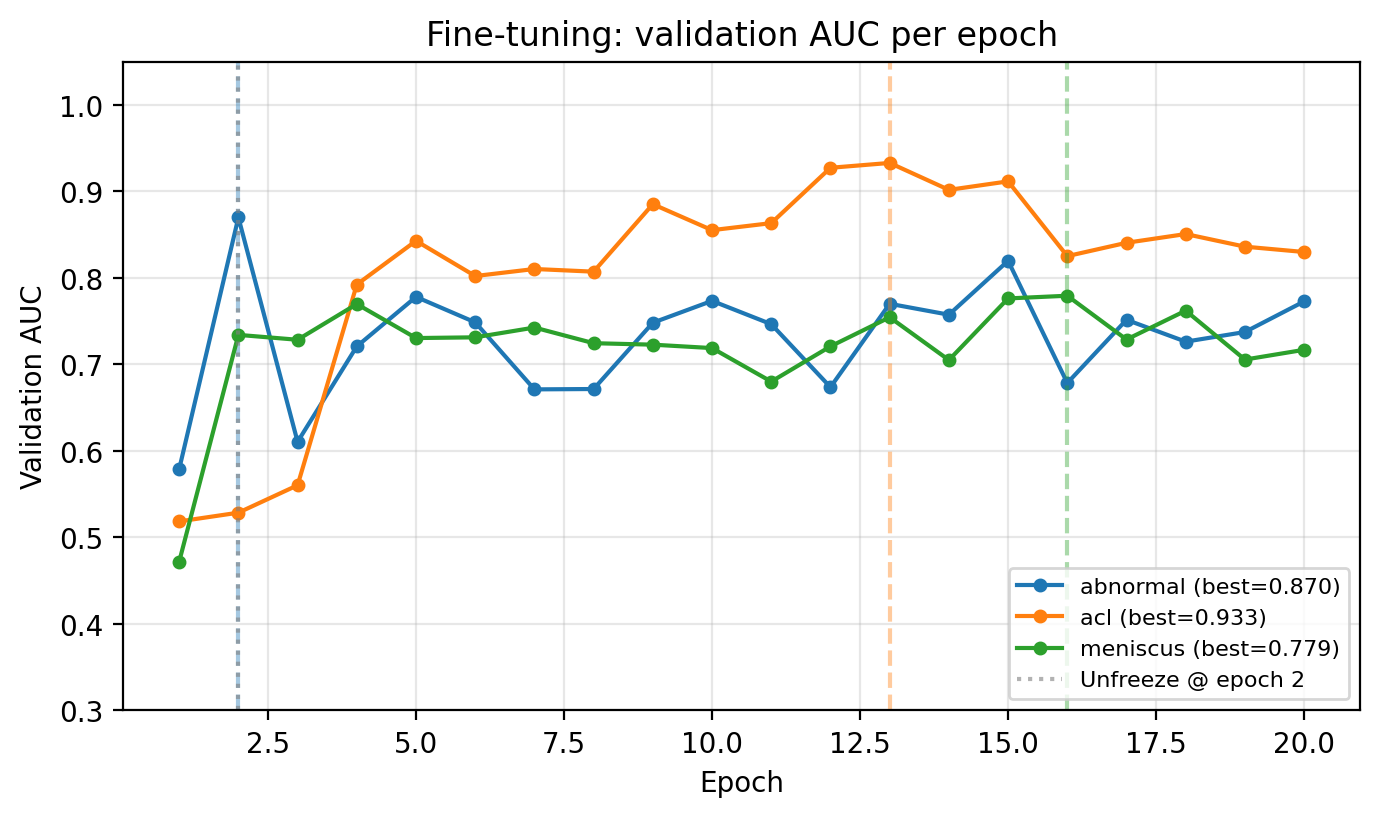
\includegraphics[width=\linewidth]{ft_valid_auc.png}
\caption{Fine-tuning: validation AUC vs.\ epoch.}
\label{fig:ft_auc_epochs}
\end{subfigure}\hfill
\begin{subfigure}{0.48\linewidth}
\centering
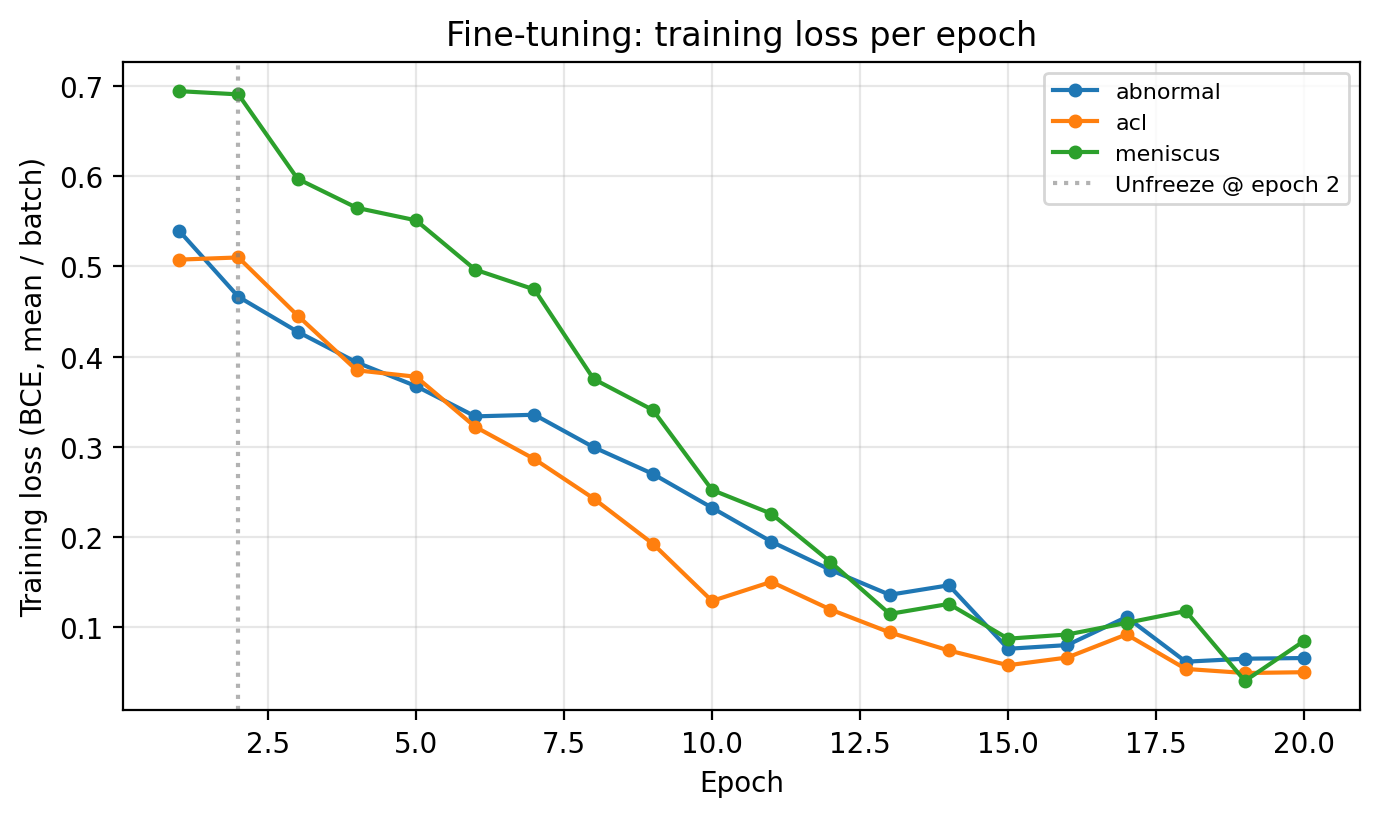
\includegraphics[width=\linewidth]{ft_train_loss.png}
\caption{Fine-tuning: training loss vs.\ epoch.}
\label{fig:ft_loss_epochs}
\end{subfigure}
\caption{Learning dynamics for the fine-tuning experiment (MRNet validation split). If these files are missing, rerun the Section~5 plot cell with \texttt{SAVE\_REPORT\_FIGURES=True}.}
\label{fig:curves}
\end{figure}

Figure~\ref{fig:to_curves} shows the same quantities for transfer-only training (backbone frozen for all epochs).

\begin{figure}[t]
\centering
\begin{subfigure}{0.48\linewidth}
\centering
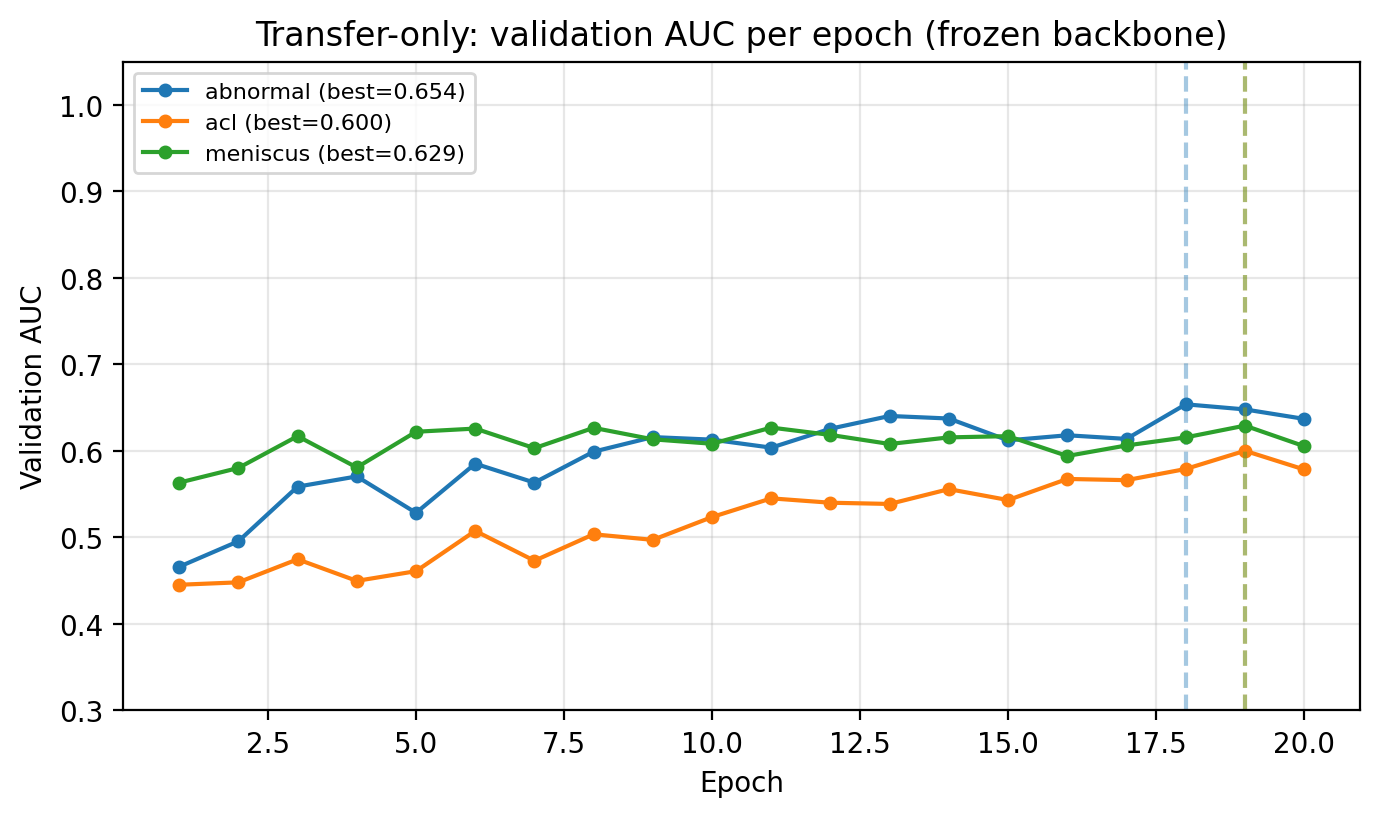
\includegraphics[width=\linewidth]{to_valid_auc.png}
\caption{Transfer-only: validation AUC vs.\ epoch (frozen backbone).}
\label{fig:to_auc_epochs}
\end{subfigure}\hfill
\begin{subfigure}{0.48\linewidth}
\centering
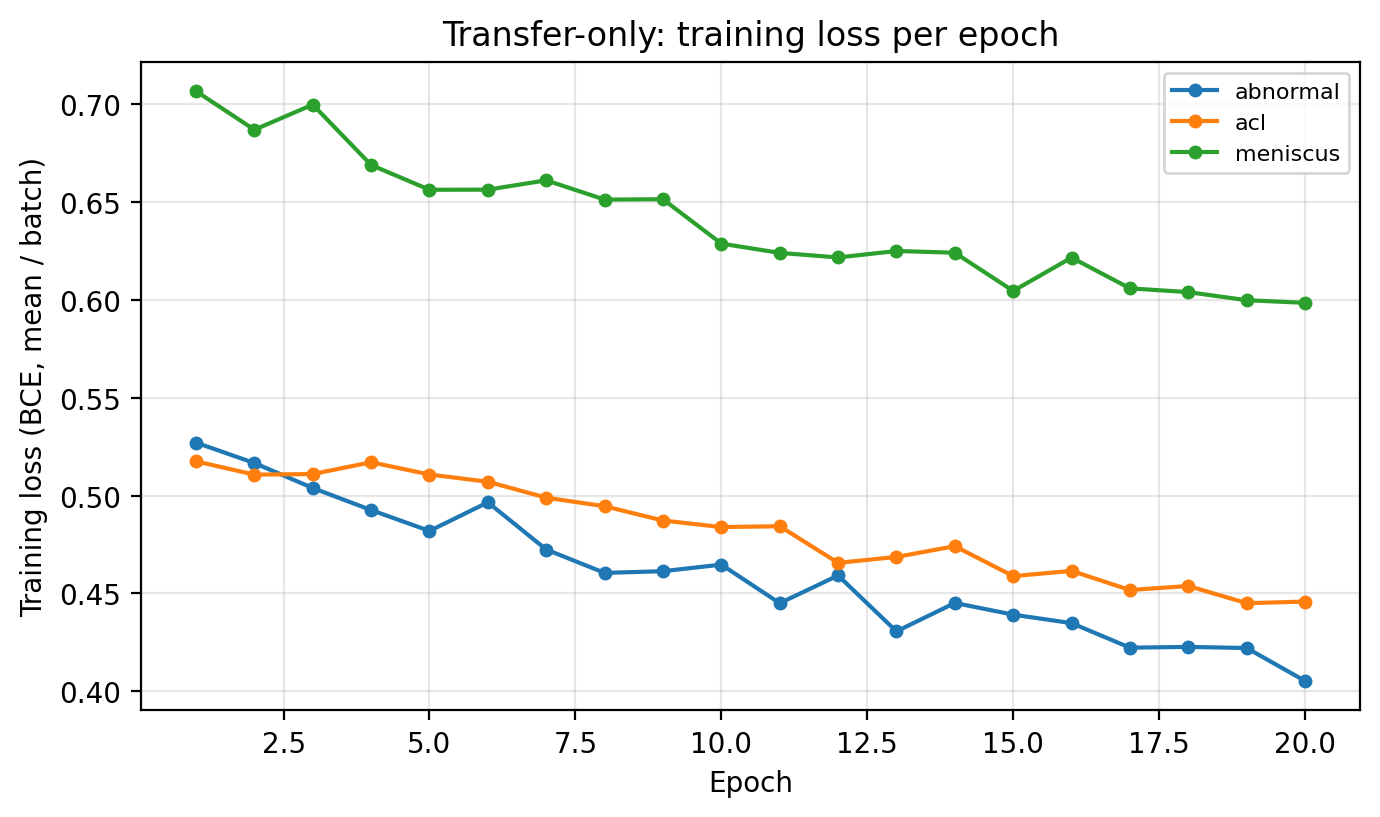
\includegraphics[width=\linewidth]{to_train_loss.png}
\caption{Transfer-only: training loss vs.\ epoch.}
\label{fig:to_loss_epochs}
\end{subfigure}
\caption{Learning dynamics when only task heads are trained (MRNet validation split).}
\label{fig:to_curves}
\end{figure}

Figure~\ref{fig:roc_pair} plots ROC curves on the MRNet validation split using the best saved checkpoint per task. Fine-tuning yields curves closer to the upper-left corner, consistent with Table~\ref{tab:auc}.

\begin{figure}[t]
\centering
\begin{subfigure}{0.48\linewidth}
\centering
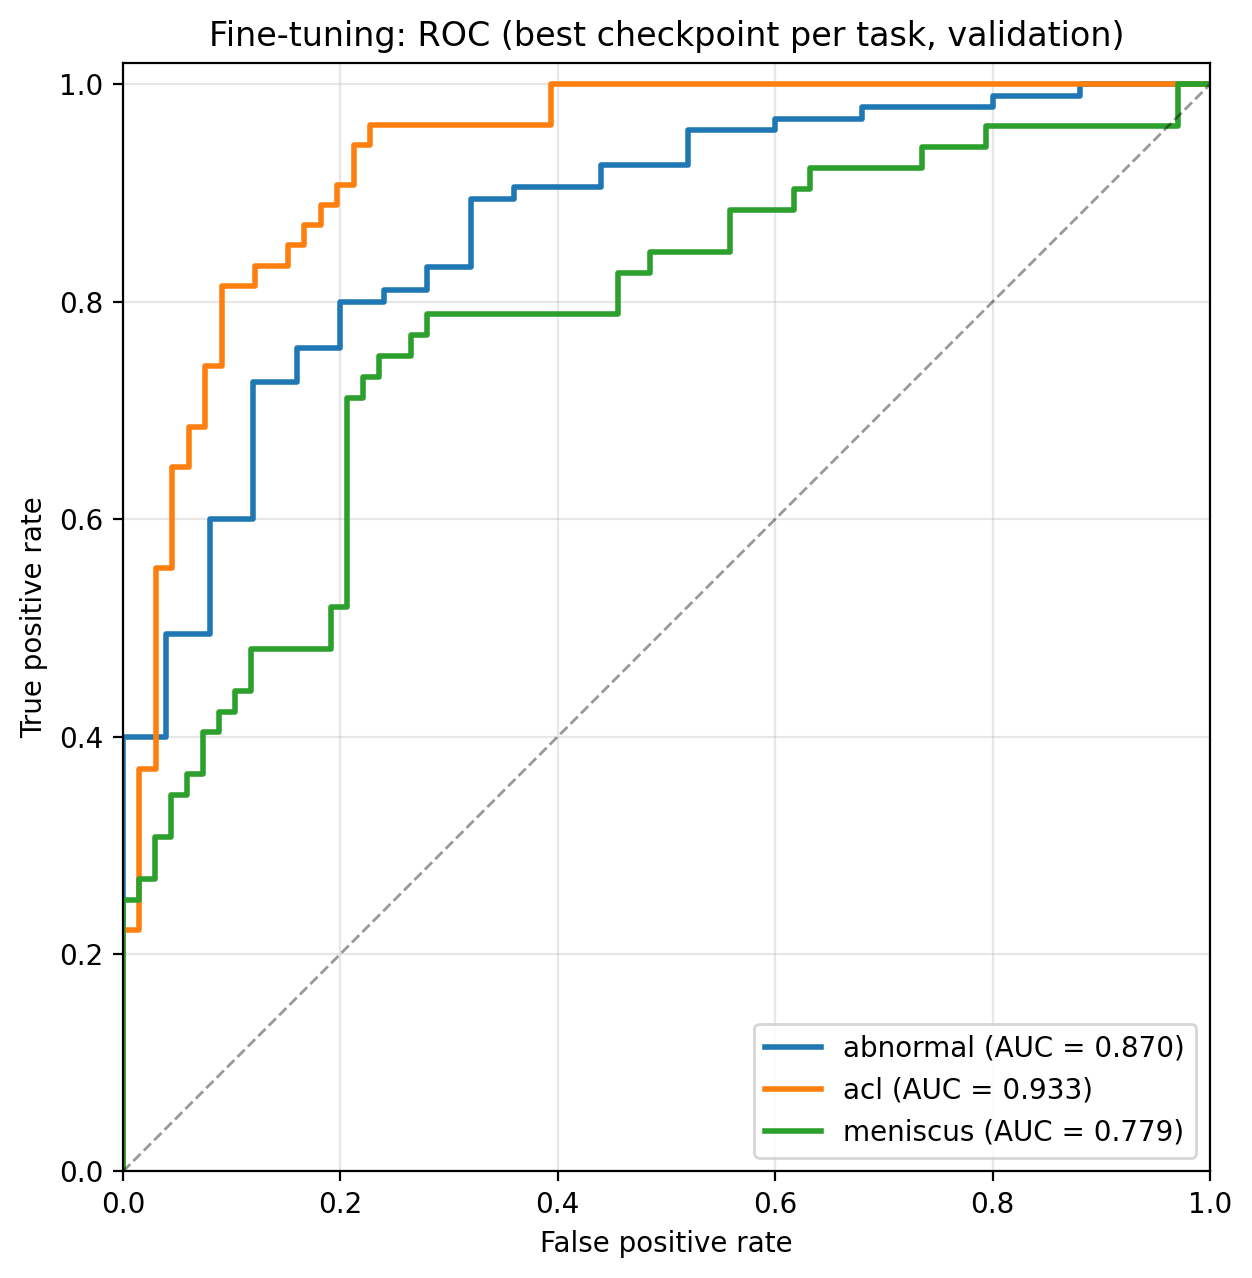
\includegraphics[width=\linewidth]{roc_finetune_validation.png}
\caption{Fine-tuning (best checkpoint per task).}
\label{fig:roc_ft}
\end{subfigure}\hfill
\begin{subfigure}{0.48\linewidth}
\centering
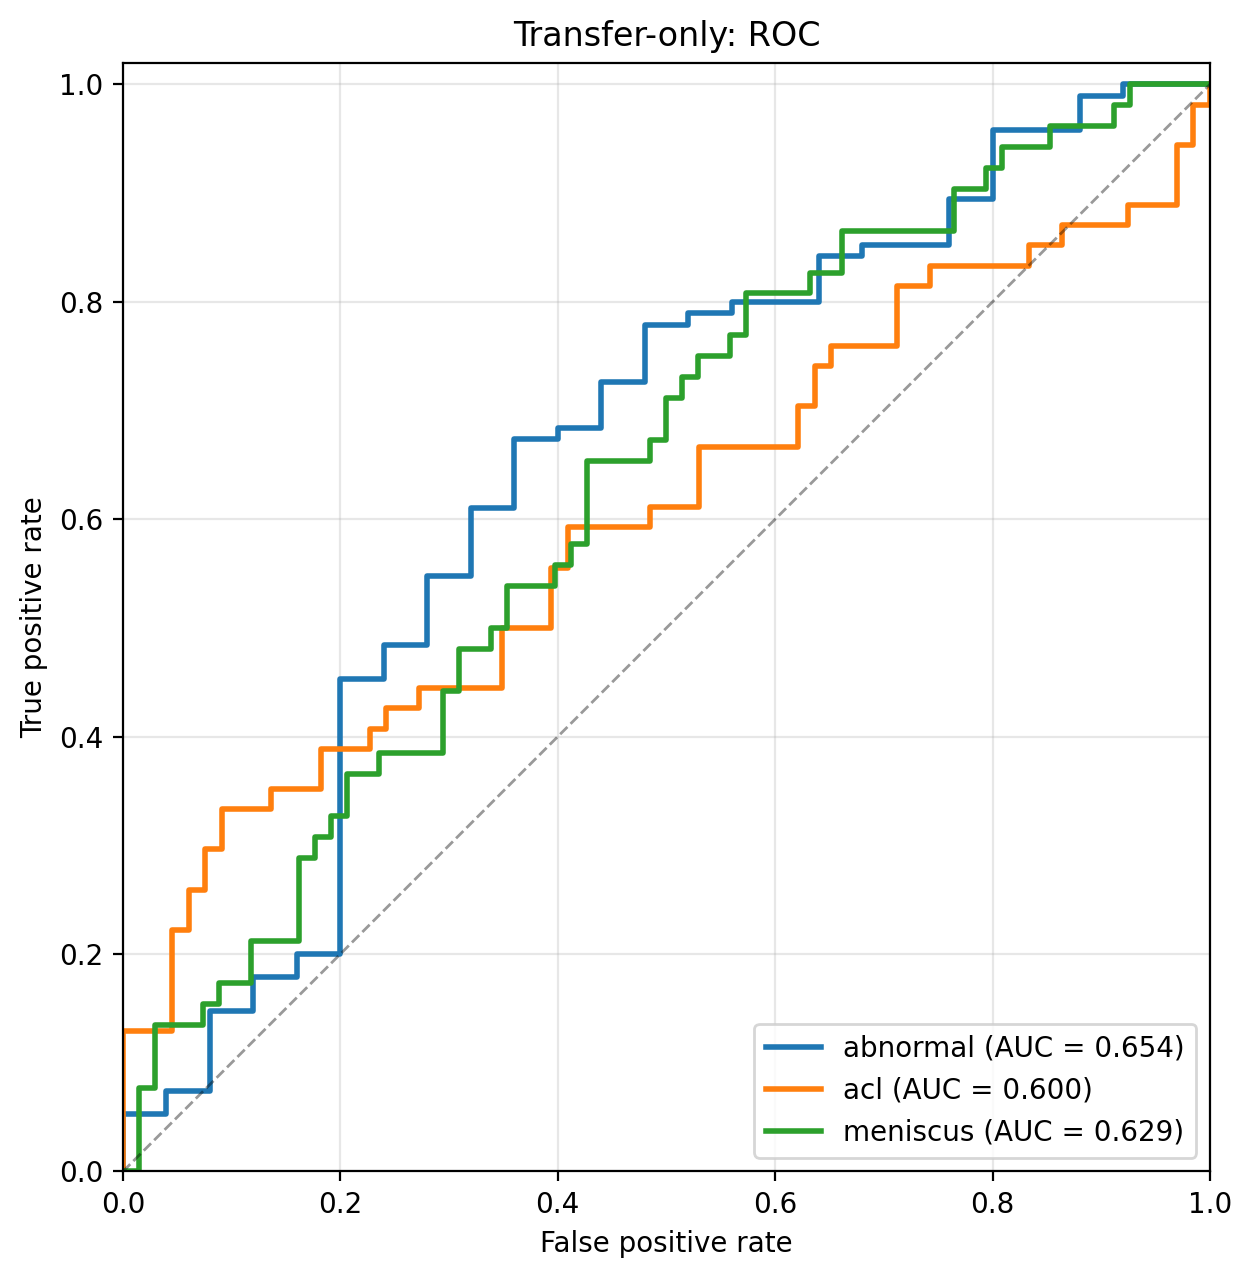
\includegraphics[width=\linewidth]{roc_transfer_only_validation.png}
\caption{Transfer-only (best checkpoint per task).}
\label{fig:roc_to}
\end{subfigure}
\caption{Validation ROC curves for all three tasks (MRNet valid split).}
\label{fig:roc_pair}
\end{figure}

Figure~\ref{fig:h2h} summarizes best validation AUC per task for both strategies.

\begin{figure}[H]
\centering
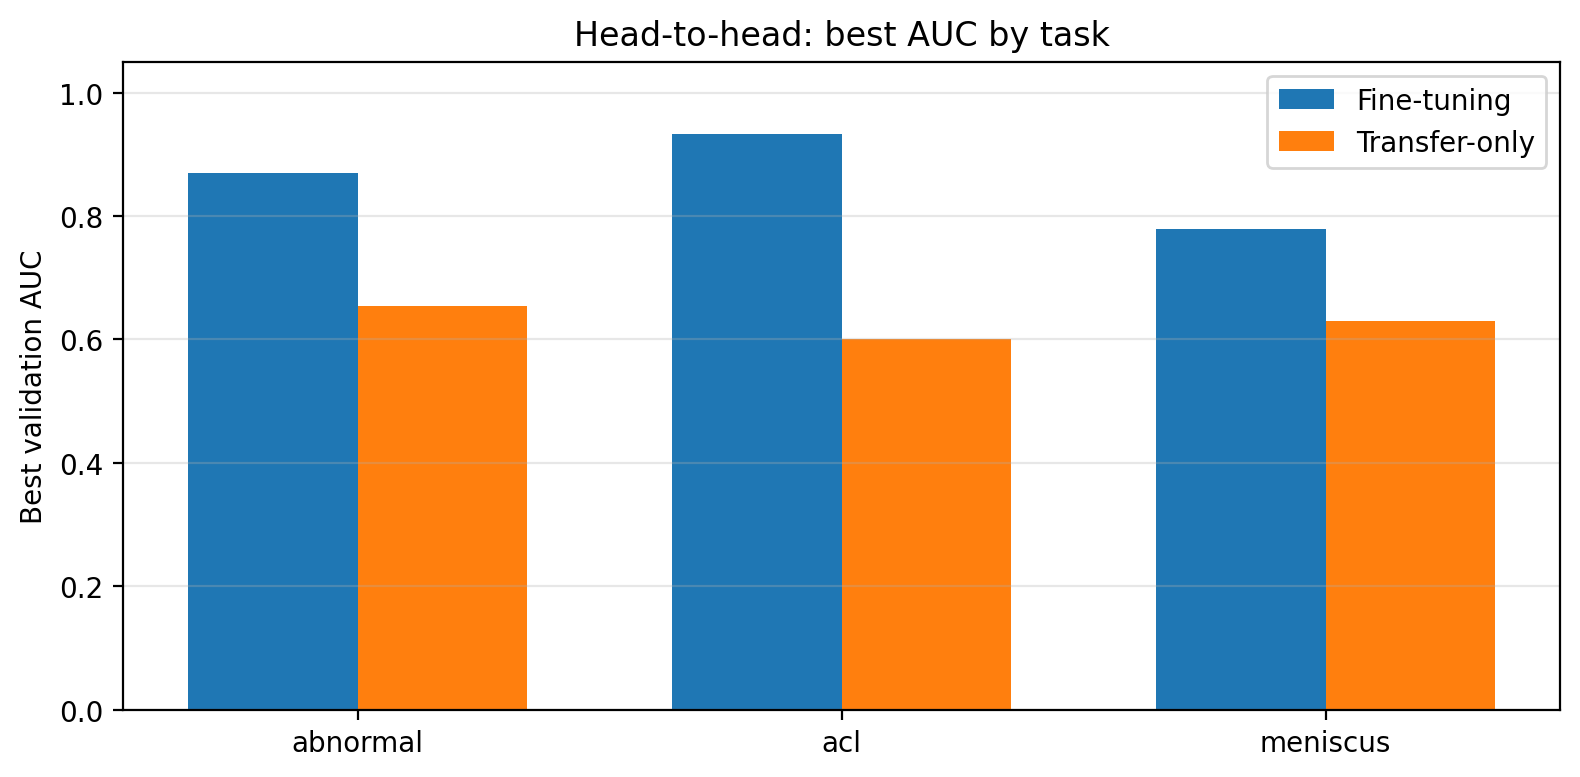
\includegraphics[width=\linewidth]{head_to_head_best_auc.png}
\caption{Head-to-head comparison of best validation AUC by task (fine-tuning vs.\ transfer-only).}
\label{fig:h2h}
\end{figure}

\subsection{Discussion}

\paragraph{Consistent benefit of fine-tuning.}
Fine-tuning improves every task, and the mean AUC gap ($\approx 0.23$) indicates the effect is not explained by a single outlier task.

\paragraph{Task-dependent margin.}
The largest improvement appears on ACL, suggesting frozen mid-level ImageNet features are least aligned with the cues needed for that label, or that the ACL decision boundary is harder to approximate with a shallow head alone. Meniscus shows the smallest gap, compatible with pretrained features retaining more transferable structure for that task---but this remains a hypothesis without layer-wise probing.

\paragraph{Overfitting and optimization.}
MRI datasets are moderately sized versus model capacity when the full backbone trains. Validation AUC that rises early then drifts downward while training loss continues to drop is compatible with increasing train-set specialization; I recommend reporting train/validation curves side-by-side where space permits.

\paragraph{Limitations.}
Single configuration and seed; noisy gradients with batch size one; no ensembling; evaluation is validation-only; class imbalance across tasks affects AUC variance; wall-clock times are hardware-dependent.

\paragraph{Key takeaways (aligned with presentation summary).}
Fine-tuning outperforms transfer-only on all three tasks. Mean validation AUC is approximately $0.861$ (fine-tune) versus $0.628$ (heads only). Per-task gaps are largest for ACL ($+0.33$) and smallest for meniscus ($+0.15$), consistent with rarity of ACL positives and partial overlap between transferable ImageNet features and each pathology's appearance.

% ============================================================================
% SECTION 5: RELATED WORK
% ============================================================================
\section{Related Work}
\label{sec:related}

Deep learning on MRNet~\cite{bien2020deep} established strong baselines for knee MRI classification. Subsequent work explores architecture variants, ensembles, and self-supervised pretraining---outside the scope of this short report.

Transfer learning from ImageNet to medical imaging is standard~\cite{deng2009imagenet, he2016deep}: natural-image pretraining often helps low-data regimes despite domain gap, especially when coupled with careful fine-tuning (learning rate freezes, discriminative LR schedules). This experiment isolates only the \textit{freeze entire training} vs.\ \textit{unfreeze after one epoch} axis under a minimal production-style training loop implemented for CECS~553.

% ============================================================================
% SECTION 6: CONCLUSION
% ============================================================================
\section{Conclusion}
\label{sec:conclusion}

I compared frozen-backbone vs.\ backbone fine-tuning for three MRNet detection tasks using a triple ResNet-18 architecture and matched training pipelines. Fine-tuning produced higher validation AUC on all tasks with a mean AUC improvement of roughly $0.23$ in the documented run---strong evidence that, under this setup, adapting pretrained convolutional weights outperforms head-only adaptation. Considering the motivating clinical constraints (throughput, consistency, rarity of some findings), the results support fine-tuning as the stronger default for this MRNet setup, with validation-only estimates understood as development metrics rather than clinical performance claims.

Future work: discriminative layer-wise learning rates; longer freezes; stochastic depth or stronger augmentation; repeating runs across seeds for confidence intervals; optional evaluation on MRNet competition test submissions if permitted.

% ============================================================================
% REFERENCES
% ============================================================================
\bibliographystyle{plain}
\begin{thebibliography}{99}

\bibitem{bien2018plos}
Nicholas Bien, Pranav Rajpurkar, Robyn L.\ Ball, et al.
\newblock Deep-learning-assisted diagnosis for knee magnetic resonance imaging: Development and retrospective validation of MRNet.
\newblock \emph{PLOS Medicine}, 15(11):e1002699, 2018.

\bibitem{bien2020deep}
Nicholas Bien, Pranav Rajpurkar, Robyn L.\ Ball, et al.
\newblock Deep-learning-assisted diagnosis for knee magnetic resonance imaging.
\newblock \emph{Radiology: Artificial Intelligence}, 2(1):e190093, 2020.
\newblock (MRNet-style knee MRI classification; see also official dataset documentation.)

\bibitem{stanford_mrnet}
Stanford AIMI.
\newblock MRNet: Knee MRIs dataset and competition resources.
\newblock \url{https://aimi.stanford.edu/datasets/mrnet-knee-mris}
\newblock (accessed 2026).

\bibitem{he2016deep}
Kaiming He, Xiangyu Zhang, Shaoqing Ren, and Jian Sun.
\newblock Deep residual learning for image recognition.
\newblock In \emph{Proceedings of the IEEE Conference on Computer Vision and Pattern Recognition (CVPR)}, pages 770--778, 2016.

\bibitem{deng2009imagenet}
Jia Deng, Wei Dong, Richard Socher, Li-Jia Li, Kai Li, and Li Fei-Fei.
\newblock ImageNet: A large-scale hierarchical image database.
\newblock In \emph{Proceedings of the IEEE Conference on Computer Vision and Pattern Recognition (CVPR)}, pages 248--255, 2009.

\bibitem{torchvision}
PyTorch maintainers.
\newblock Torchvision model zoo (ResNet-18 ImageNet weights).
\newblock \url{https://pytorch.org/vision/stable/models.html}

\bibitem{requirements}
Project \texttt{requirements.txt}: PyTorch, torchvision, NumPy, pandas, scikit-learn, tqdm, matplotlib.
\newblock \texttt{github.com} student project repository (CECS 553), 2026.

\end{thebibliography}

\end{document}
